% This is a very simple Latex example
%
% This first bit is commented out

\documentclass[a4paper,11pt]{article}

\usepackage{epsf,epsfig,amsfonts} % allows epsfig comands
%\usepackage {html} % allows html links to be added
\usepackage{multicol}  % allows use of multi-columns within a page
\usepackage{times}     % space-saving font
\usepackage{color}     % allows colour fonts
\usepackage{bm}

\textheight 25.0cm
\textwidth 16cm
\topmargin -1.5cm
\oddsidemargin -0cm


%\pagestyle{plain}

% These are some ``macro'' defintions

\def\apj{{ApJ.}}
\def\apjs{{ApJS.}}
\def\apjl{{ApJL.}}
\def\nat{{Nature.}}
\def\mnras{{MNRAS}}
\def\araa{{ARA\&A}}
\def\aap{{A\&A}}
\def\aj{{AJ}}
\def\aaps{{A\&AS}}
\def\apss{{Ap\&SS}}

\def\spose#1{\hbox to 0pt{#1\hss}}
\def\simlt{\mathrel{\spose{\lower 3pt\hbox{$\mathchar"218$}}
     \raise 2.0pt\hbox{$\mathchar"13C$}}}
\def\simgt{\mathrel{\spose{\lower 3pt\hbox{$\mathchar"218$}}
     \raise 2.0pt\hbox{$\mathchar"13E$}}}

% itemz environment: Like itemize but waste less space
 \newenvironment{itemz}
 {\begin{list}{$\bullet$}{\setlength{\itemsep}{0pt}}}
 {\end{list}}



% Setting up some stuff that will go into the title
\author{Seb Oliver, Peter Hurley}
\title{HELP: FIR Luminosity Function from a map}
\date{July 11th 2014}

% Now we start doing some stuff

\begin{document}

% This is where the title is written
\maketitle

\tableofcontents
%\listoffigures
%\listoftables


\section{Introduction}
An important approach in the understanding of the evolution of galaxy populations is to compare statistical summaries of populations at different redshifts.    Luminosity functions are a pretty ubiquitous example.
Determining the far Infrared luminosity function is an important one.  FIR data suffers from large beams.  But there is lots of information in the map.  So we'd like to get the Luminosity function directly from the map.  Here we explore how to do that using Bayesian probabilistic modelling approach.

\section{What data are we going to use?} 
As a simple example lets assume that we have (i) a far infrared map with surface brightness $B_{\rm IR}$ as a function of sky position $(\alpha, \delta)$, this can be represented as a data vector $\mathbf{B}$  (ii) a spectroscopic redshift catalogue given exact redshifts $z_j$ for a set of galaxies that have a optical fluxes $f_{\rm opt}$ satisfying some threshold criteria.   

We also know things like the FIR beam and the selection functions of the data sets.

\section{What are we interested in?}
We principle want to know the luminosity function $\psi(L_{\rm IR},z)$ which gives the number density of galaxies i.e. is defined by 
$$dN=\psi( L_{\rm IR},z)\,d\log L_{\rm IR}\,dV=\psi( L_{\rm IR},z)\,d\log L_{\rm IR}\,\frac{dV}{dz\,d\Omega}\,dz\,d\Omega.$$

In practice we are need to know (and might also be interested in) the bivariate luminosity function

$$\psi( L_{\rm IR},L_{\rm opt},z),$$
defined in a similar way.

These luminosity functions can be parameterised in many ways.  We will likely be wanting to parameterise as parametric functions in luminosity and step-functions in $z$.  The parameter set to define the luminosity function is $\bm{\theta}$

Because we worship at the altar of Bayes we want to turn the luminosity function into a probability density, 
$$P(\log L_{\rm IR},\log L_{\rm opt},\bm{r}),$$ being the probability density of finding a galaxy at position $\bm{r}$ with $L_{\rm IR}$ and $L_{\rm opt}$, which is defined such that the probability of finding a galaxy in the interval $d\log L_{\rm IR}\,d\log L_{\rm opt}\, d \bm{r}$
$$dP=P(\log L_{\rm IR},\log L_{\rm opt},\bm{r}) d\log L_{\rm IR}\,d\log L_{\rm opt}\,d\bm{r}$$
Noting that $d\bm{r}=dV$ and that $dP = dN$ in the infinitesimal limit we see that 
$$P(\log L_{\rm IR},\log L_{\rm opt},\bm{r})=\psi( L_{\rm IR},L_{\rm opt},z)$$

\section{Optical Selection}
Assume that we have a galaxy with the following properties: $\log L_{\rm IR},\log L_{\rm opt},\bm{r}$.
A crucial consideration is the optical selection. This is the probability that the galaxy was in the original optical catalogue and then that the galaxy obtained a spectroscopic redshift. 

Given that the galaxy is in the parent optical photometric catalogue...The spectroscopic redshift success will likely depend on the redshift survey geometry and the redshift of the galaxy and the flux of the galaxy. Let's assume that the probability of having a spectroscopic redshift is simply a function of the true optical flux, $f_{\rm opt}$, angular position and redshifts$ \bm{r}$.  I.e. the probability of the galaxy being in our redshift sample, $P({\rm zcat})$, is defined by a {\em selection function}:
$$P({\rm zcat}| f_{\rm opt}, \bm{r}, {\rm photcat}).$$  

In the simple case that we have a single galaxy type with a known spectral energy distribution there will be a deterministic function that relates to the ``true'' optical flux, $f_{\rm opt}$, to the luminosity and redshift i.e.
$f_{\rm opt}=f(\log L_{\rm IR},\log L_{\rm opt},\bm{r})$.

The original optical photometric survey produces a catalogue of observed fluxes There will then be another probabilistic {\em selection function} which relates the observed flux to the ``true" flux, which may also depend on position i.e.,
$$ P(f_{\rm opt}^\prime|f_{\rm opt},\bm{r})$$

also need the probability that the object would be in the photometric catalogue which is probably a simple function of its observed flux

$$P({\rm photcat}| f_{\rm opt}^\prime)$$

\section{Bayesian Inference}
To get a better handle on how variables and observables are related, we can create a graphical model. Figure \ref{fig:graph_model} shows our graphical model for getting $$P(\log L_{\rm IR},\log L_{\rm opt},\bm{r}),$$
$A_i^j$ denotes the contribution from source $i$ at pixel $j$, while $m_j$ is our model flux at pixel $j$. Other variables are as described above.

\begin{figure}
\centering
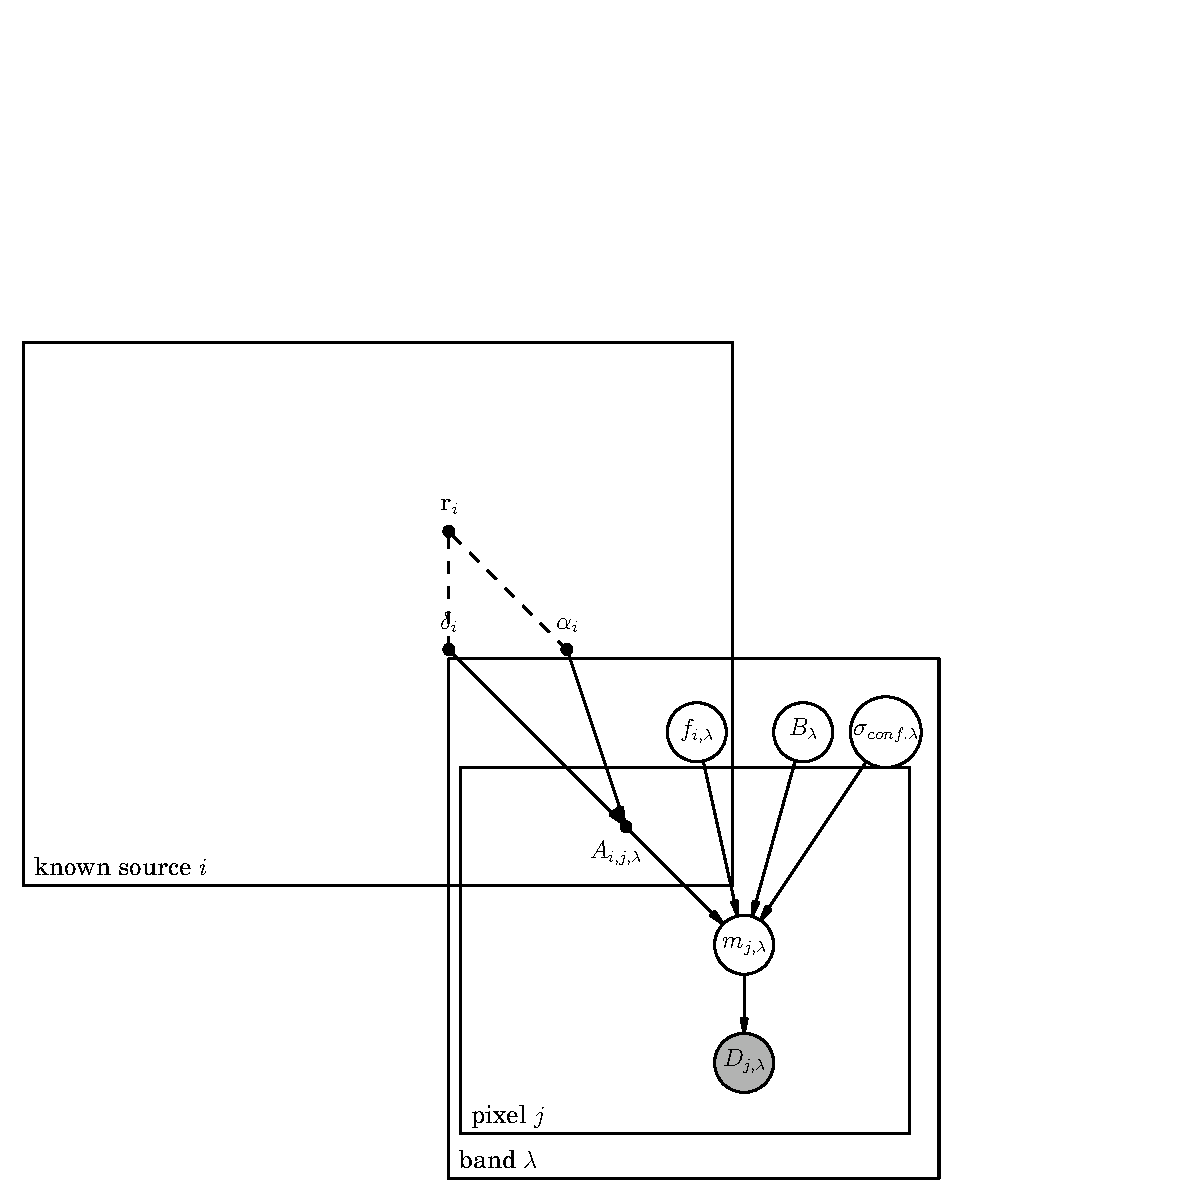
\includegraphics{graphical_model.pdf}
\caption{Graphical model for luminosity function. Dashed lines represent deterministic links, while solid lines represent probabilistic connections. Fixed variables are plotted as blobs, open circles as variables, and shaded circles as observed variables.}\label{fig:graph_model}
\end{figure}

Now we have the basic assumptions as to how variables interact with each other (i.e. the probabilistic model is constructed) all questions of interest are answered by performing inference on the distribution. 
\end{document}



